\section{Corroboration and results}
\label{corroboration_results}

% -----------------------------------------------------------------------------
% Methodology

\subsection{Methodology}

Two formulations were used to corroborate the results of the XFEM implementation.

Equation \ref{eq:interface-error} computes the difference in solutions at the discontinuity. Since the model we have implemented is based on inclusions and not crack propagation, this interface error should approach zero as the mesh gets finer.
%
\begin{equation}
	\sqrt{\frac{\sum_{\mathrm{element}} \sum_{\mathrm{interface}} \int u^+-u^- \mathrm{d}\Gamma_i}{\sum_{\mathrm{element}} \sum_{\mathrm{interface}} \int \mathrm{d}\Gamma_i}}
	\label{eq:interface-error}
\end{equation}

This equation computes the interface ``jump'' across all interfaces and elements in the model, then scales it with respect to the perimeter or area of the interface, and finally takes the square root.

Equation \ref{eq:L2-error} compares the relative difference between the XFEM solution and the FEM solution.
%
\begin{equation}
	\sqrt{\frac{\int u_{\mathrm{XFEM}}-u_{\mathrm{FEM}} \mathrm{d}\Omega}{\int u_{\mathrm{FEM}} \mathrm{d}\Omega}}
	\label{eq:L2-error}
\end{equation}

$u_{\mathrm{XFEM}}$ represents the XFEM solution, while $u_{\mathrm{FEM}}$ represents the FEM solution.

XFEM was used to solve a thermal problem with the configuration of Figure \ref{fig:thermal-setup}. The same problem was ran using the classical FEM. The FEM problem used two different types of elements and its mesh was refined until the solution reached convergence.
%
\begin{figure}[htbp]
	\centering
	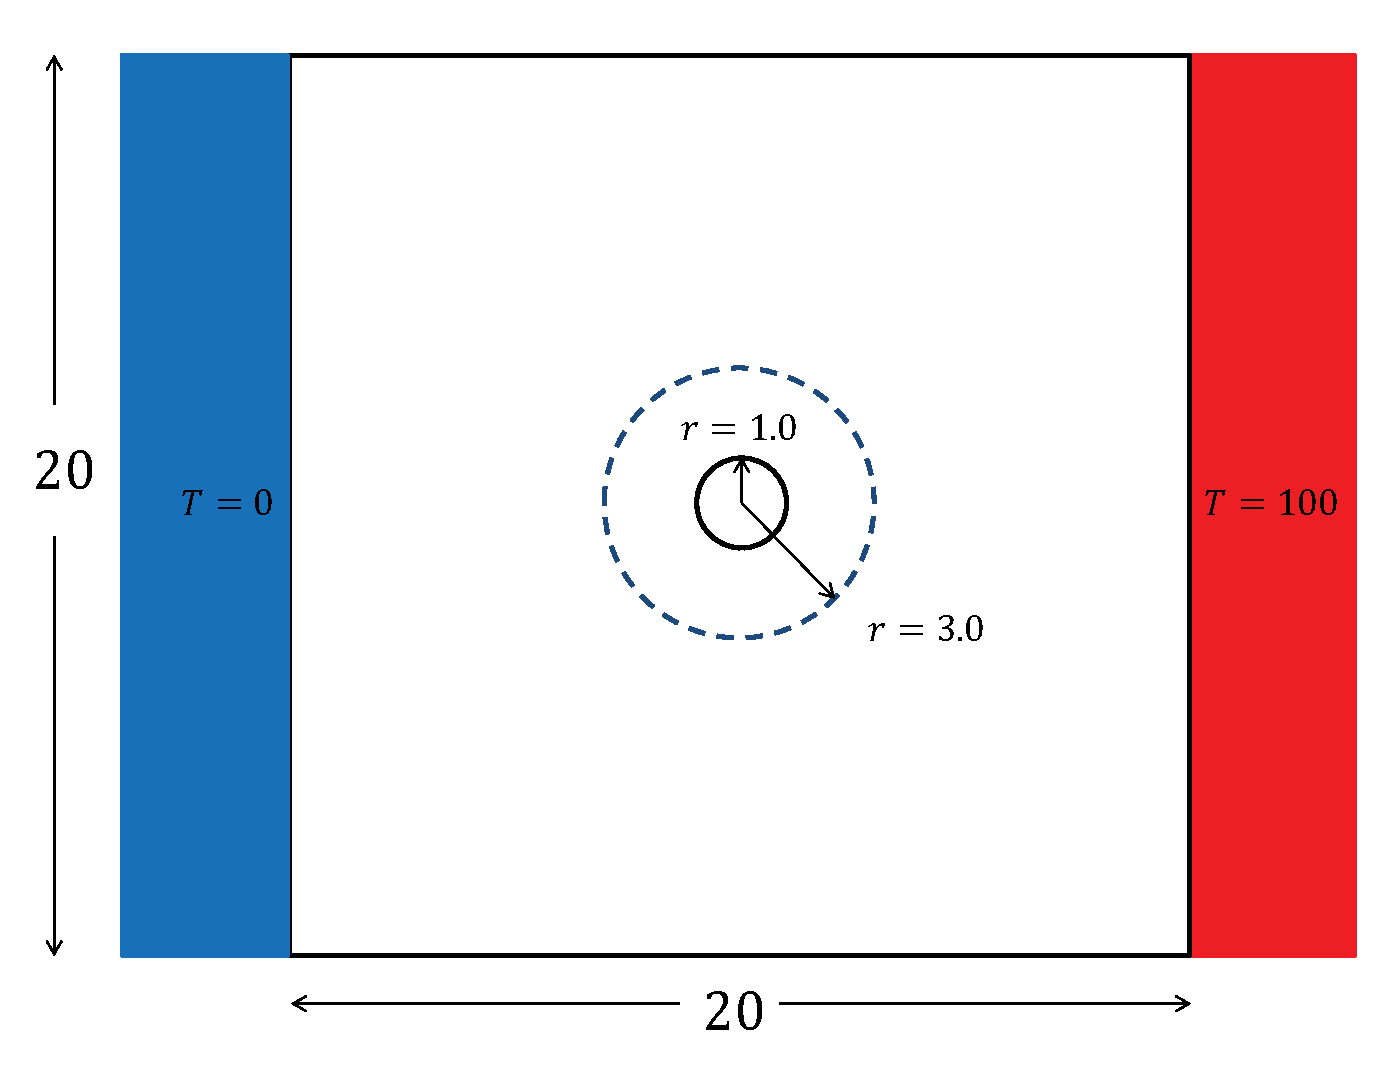
\includegraphics[width=0.75\linewidth]{diffusion_setup.eps}
	\caption[Diffusion problem setup]{Diffusion problem setup.}
	\label{fig:thermal-setup}
\end{figure}

The mesh has a width of $20$ units and a height of $20$ units. The problem has Dirichlet boundary conditions on the sides. The temperature is prescribed to $0$ on the left side and $100$ on the right side. There is an inclusion at the center of the model. This inclusion is a different material with a different thermal conductivity than the material phase $1$ domain.

The test consisted in modifying the diameter of the circle from $2$ units to $6$ units in $500$ steps using different mesh refinements, different conductivity ratios and different preconditioners formulations.

% -----------------------------------------------------------------------------
% Tests

\subsection{Tests}

% -----------------------------------------------------------------------------
% Mesh refinement

\subsubsection{Mesh refinement sweep}

The mesh size was the variable in this test, while the conductivity ratio between both materials remained fixed at 10. No preconditioner scaling was applied. The different mesh sizes used were $20 \times 20$, $30 \times 30$, $40 \times 40$, and $50 \times 50$.

Figure \ref{fig:mesh-sweep-interface} shows that as the mesh is refined, the interface error converges to zero.

\begin{figure}[H]
	\centering
	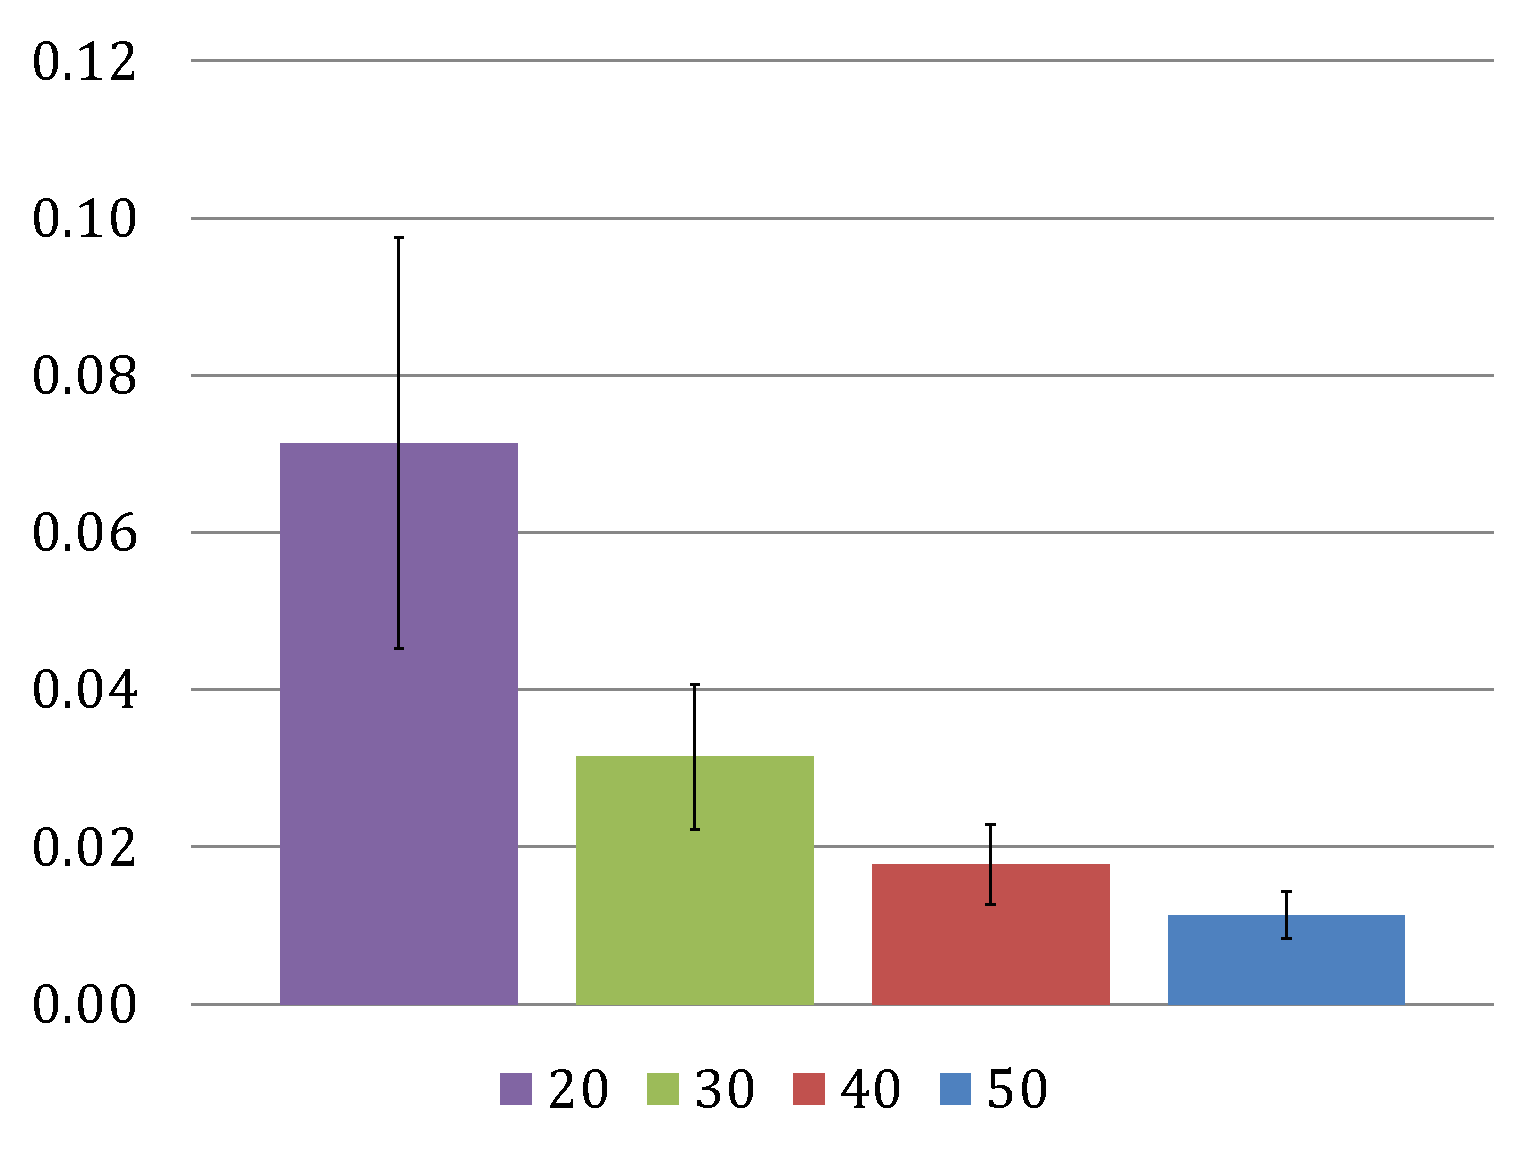
\includegraphics[width=0.5\linewidth]{mesh_sweep_interface.eps}
	\caption[Mesh refinement sweep interface error]{Mesh refinement sweep interface error.}
	\label{fig:mesh-sweep-interface}
\end{figure}

Figure \ref{fig:mesh-sweep-L2} shows that as the mesh is refined, the difference of the XFEM solution with respect to the FEM solution decreases. The larger difference for the $50 \times 50$ mesh is due to the sampling and different mesh sizes used for the XFEM and FEM problems. A different mesh resampling size fixed the issue in other tests.
%
\begin{figure}[H]
	\centering
	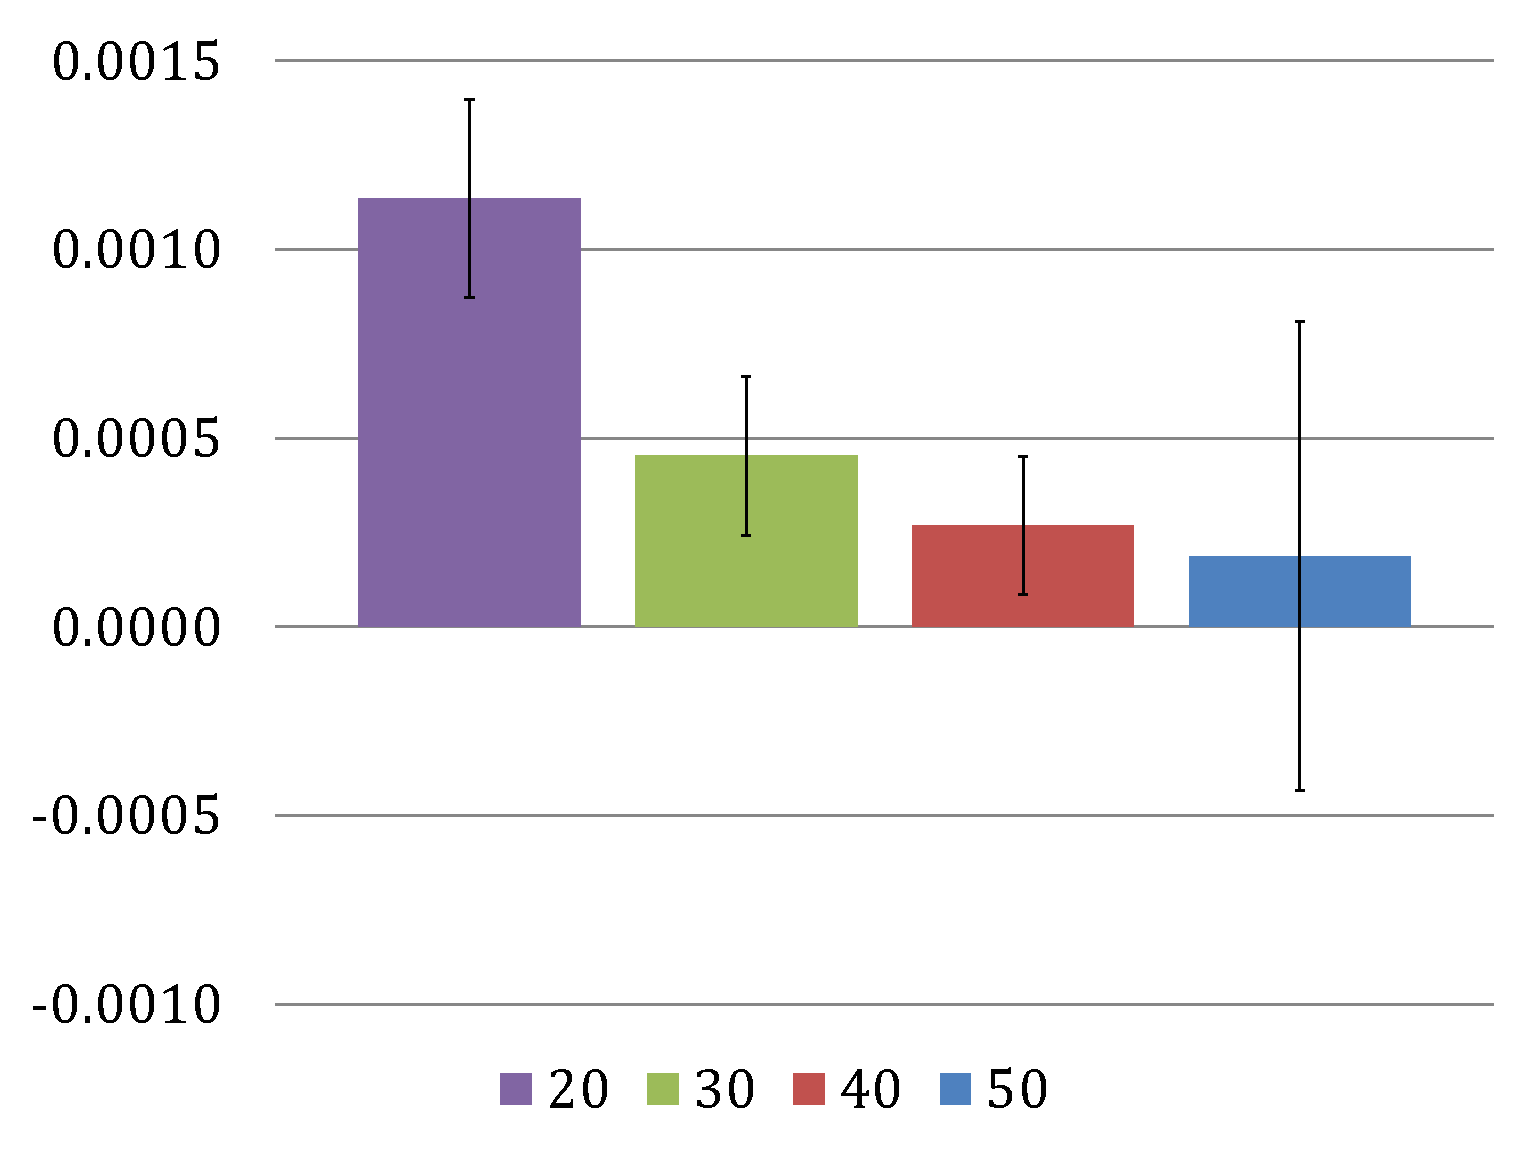
\includegraphics[width=0.5\linewidth]{mesh_sweep_L2.eps}
	\caption[Mesh refinement sweep L2 error]{Mesh refinement sweep L2 error.}
	\label{fig:mesh-sweep-L2}
\end{figure}
%
% -----------------------------------------------------------------------------

\subsubsection{Conductivity ratio sweep}

The conductivity ratio between the different materials was the variable in this test. The mesh size was $30 \times 30$ and the preconditioner formulation used the maximum spatial derivative of the shape functions. The different conductivity ratios used were 0.1, 10, 100, and 1000.

Figure \ref{fig:conductivity-sweep-interface} shows that when the material conductivity is the same for both materials (a ``quasi-FEM'' problem), the interface error is in the order of $O(\epsilon)$. However, the greater the difference in material properties at an interface, the larger the interface jump is.
%
\begin{figure}[H]
	\centering
	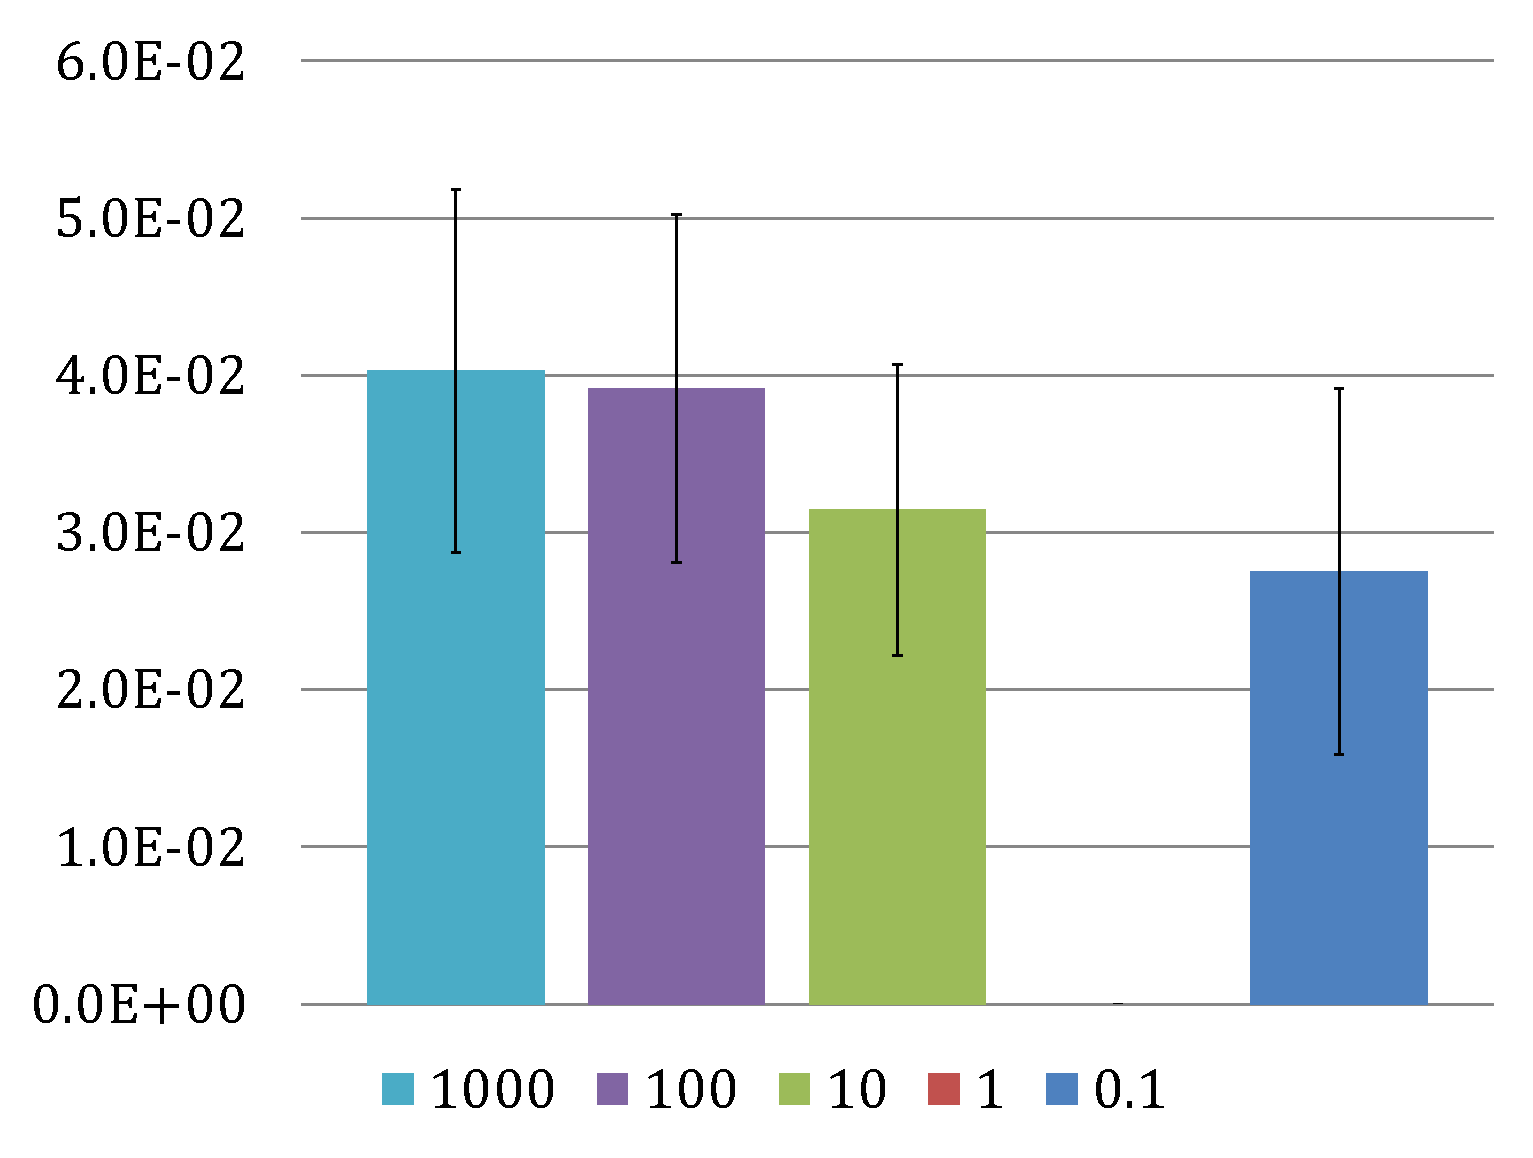
\includegraphics[width=0.5\linewidth]{conductivity_sweep_interface.eps}
	\caption[Conductivity refinement sweep interface error]{Conductivity refinement sweep interface error.}
	\label{fig:conductivity-sweep-interface}
\end{figure}

For the L2 computation, only FEM solutions with conductivity ratios of 10, 100, and 1000 were computed. Figure \ref{fig:conductivity-sweep-L2} shows that the difference in solutions is very small ~$O(10^{-4})$.
%
\begin{figure}[H]
	\centering
	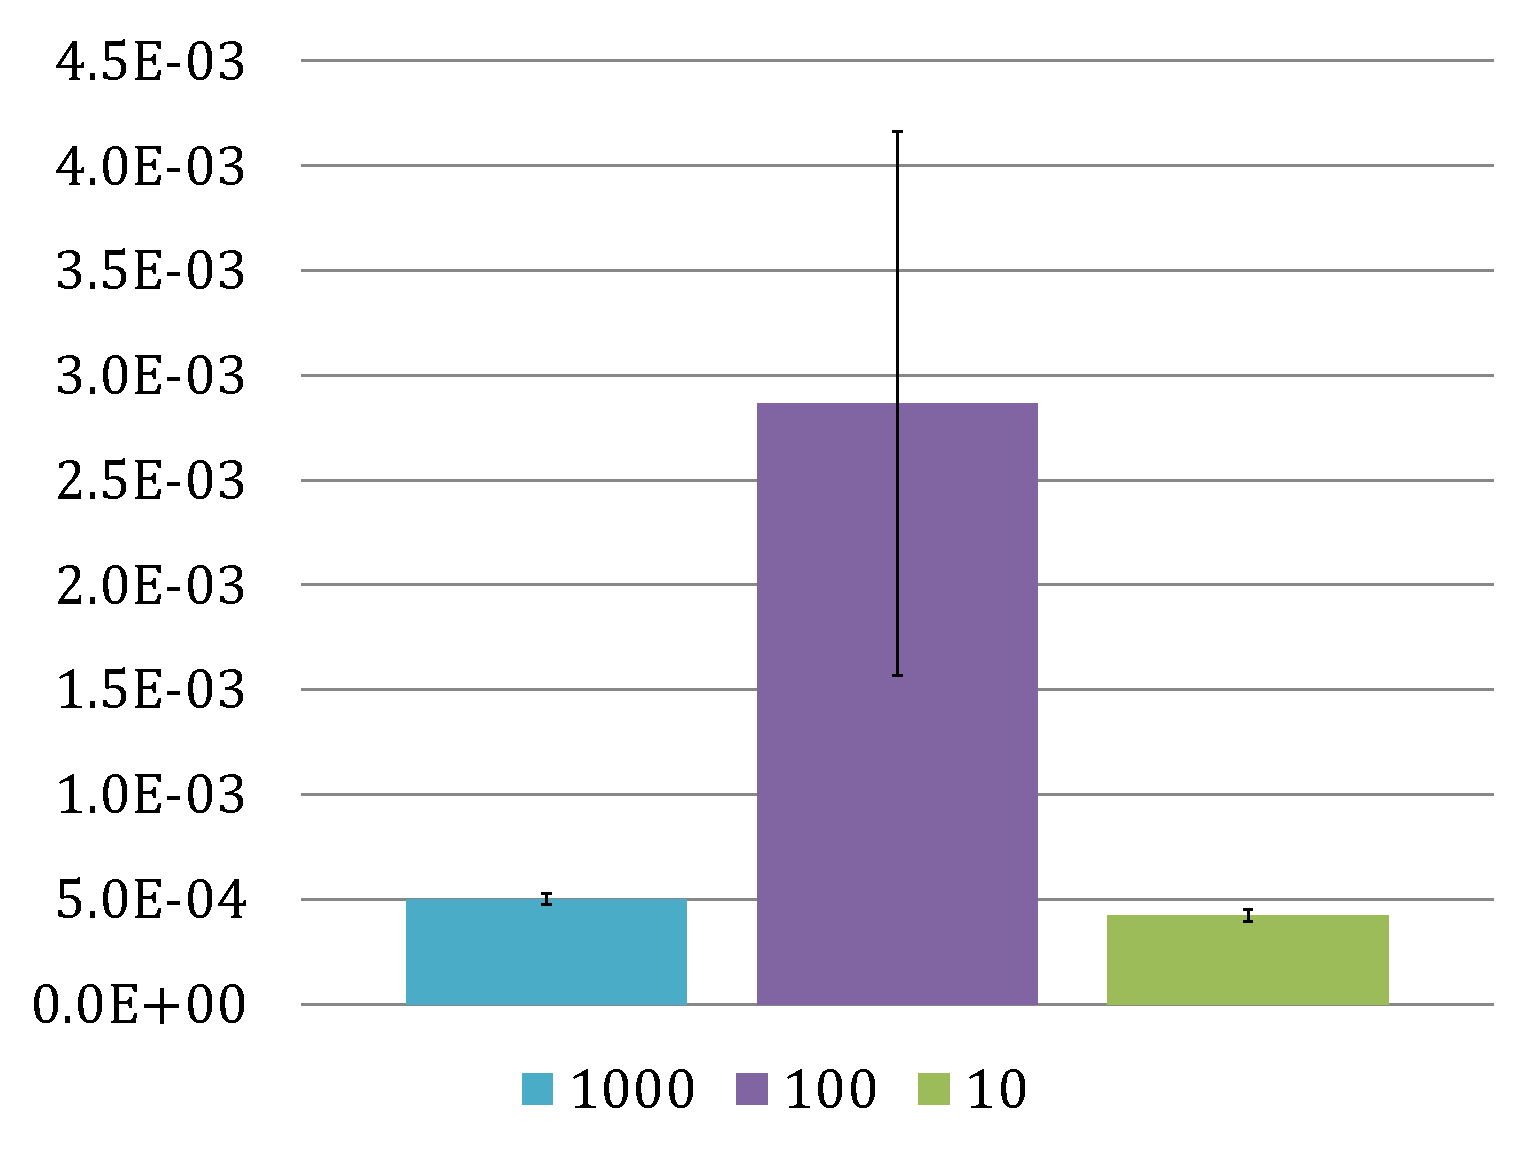
\includegraphics[width=0.5\linewidth]{conductivity_sweep_L2.eps}
	\caption[Conductivity refinement sweep L2 error]{Conductivity refinement sweep L2 error.}
	\label{fig:conductivity-sweep-L2}
\end{figure}
%
% -----------------------------------------------------------------------------

\subsubsection{Condition number comparison}

These tests were performed to compare the condition number of the global Jacobian matrix when the scaling was applied. The mesh size was $30 \times 30$, the conductivity ratio was 10 and the preconditioner formulation used the maximum spatial derivative of the shape functions. A direct solver and a GMRES iterative solver were used and compared.

Figure \ref{fig:condition_number_no_scaling} shows that the Jacobian matrix has a condition number in the order of $10^{15}$ when no scaling is applied \footnote{We use the GMRES solver provided by the Trilinos linear algebra package to solve for the linear system. The solver uses an ILU preconditioner on top of the XFEM preconditioner of this study. However, the condition number of the matrix, after the ILU preconditioner is applied, is not provided by the Trilinos package. Because of that, the direct and iterative solver yield the same condition number. In reality, the GMRES option may have a lower condition number due to the ILU preconditioner.}, while Figure \ref{fig:condition_number_scaling} shows that the condition number decreases to the order of $10^4$ when scaling is applied.
%
\begin{figure}[htbp]
	\centering
	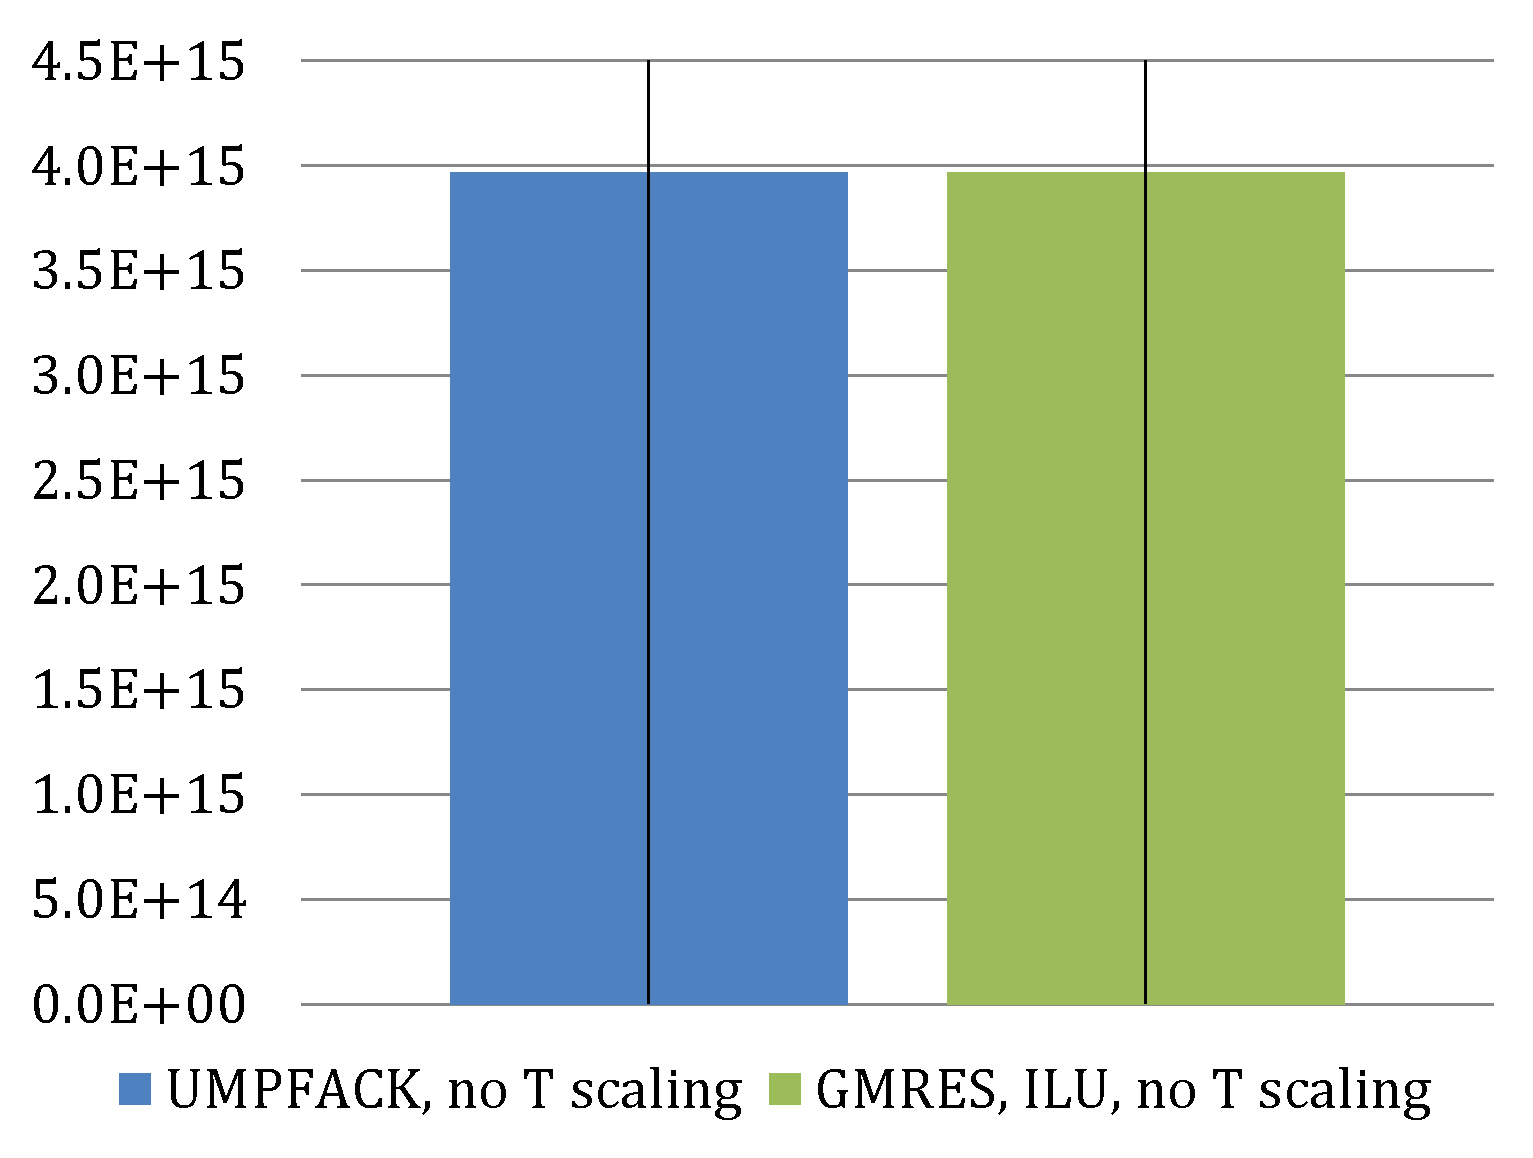
\includegraphics[width=0.5\linewidth]{condition_number_no_scaling.eps}
	\caption[Condition number comparison - no preconditioner]{Condition number comparison - no pre-conditioner.}
	\label{fig:condition_number_no_scaling}
\end{figure}
%
\begin{figure}[htbp]
	\centering
	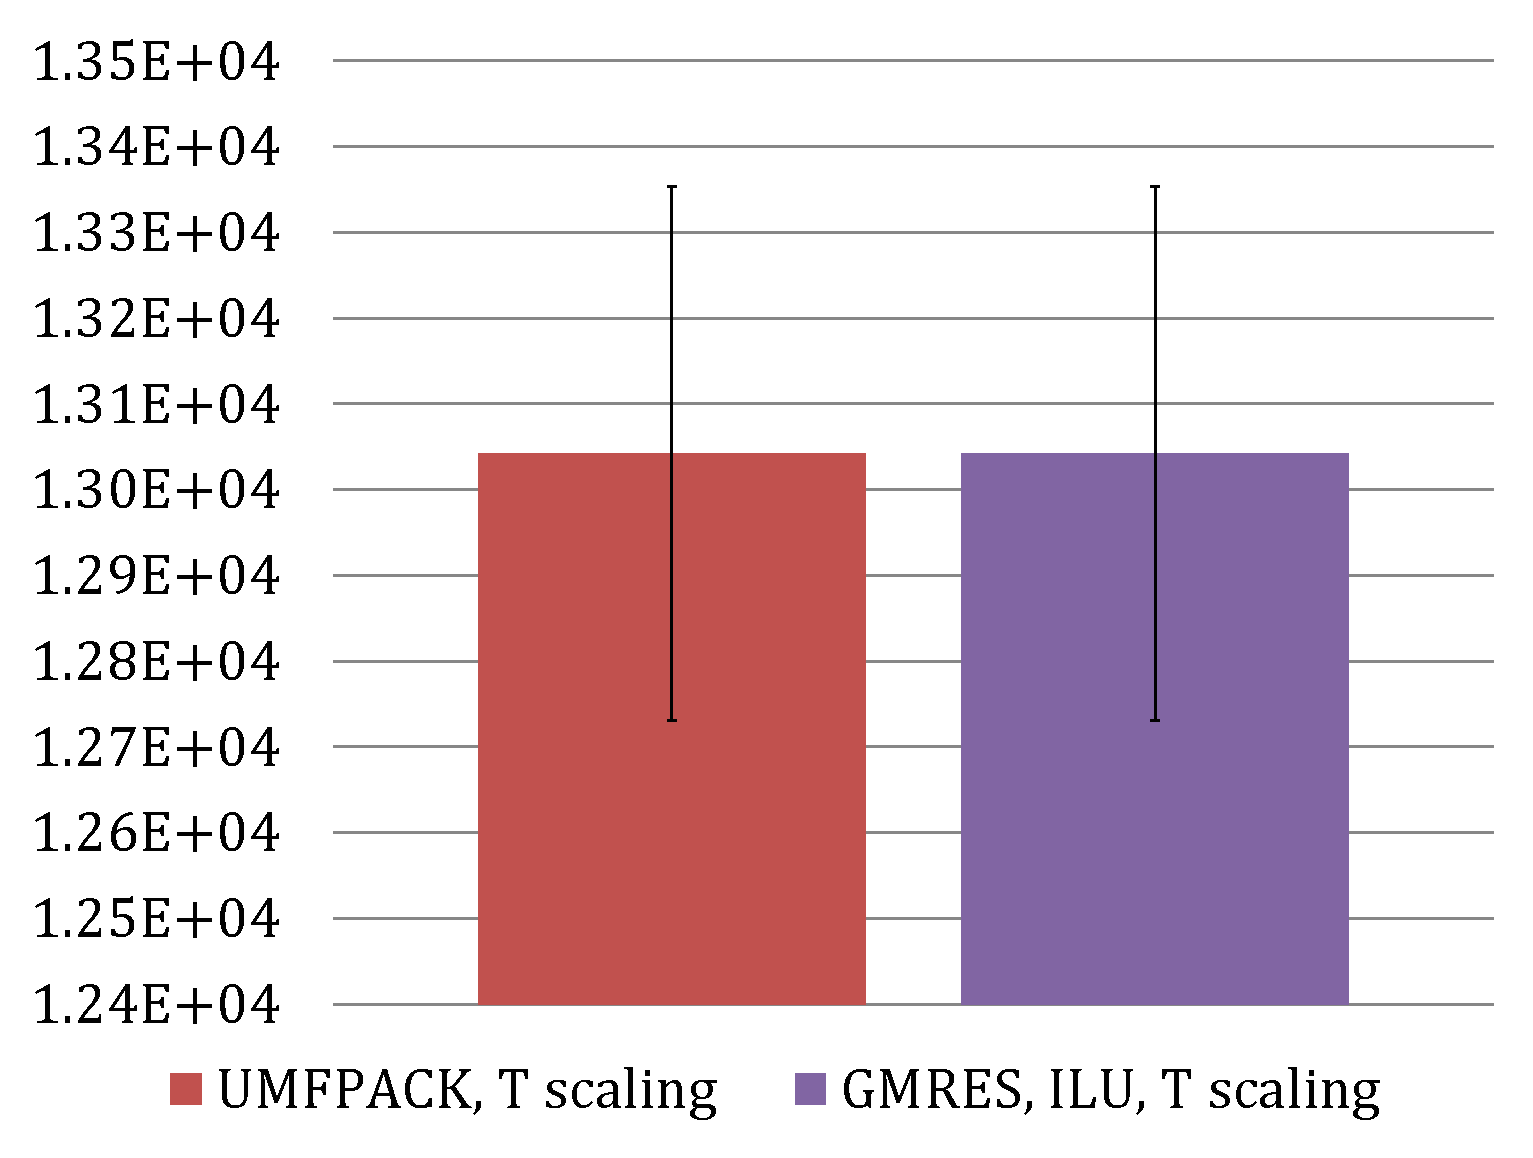
\includegraphics[width=0.5\linewidth]{condition_number_scaling.eps}
	\caption[Condition number comparison - with preconditioner]{Condition number comparison - with pre-conditioner.}
	\label{fig:condition_number_scaling}
\end{figure}